\documentclass[tikz,10pt]{standalone}
\usepackage{amsmath,amssymb,cmap,pgfplots,pgfplotstable}
\usetikzlibrary{arrows,calc,intersections}
\pgfplotsset{compat=newest}

\begin{document} 
	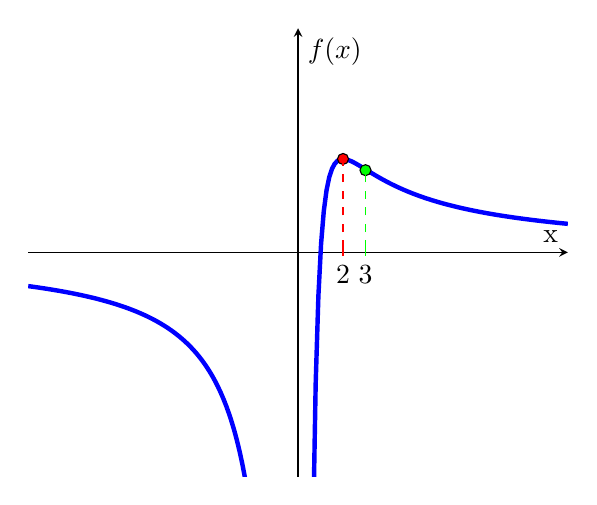
\begin{tikzpicture}
		\begin{axis}[xlabel=x, ylabel={$f(x)$}, axis lines=middle, ymax = 0.5, ymin = -0.5, xmax = 10,	xmin = -10, enlargelimits=true,xtick=\empty,	ytick=\empty, restrict y to domain=-2:2]
			\addplot[blue!, line width=1.6pt,	domain={-12:12}, samples=200]{1/x-1/x^2};
			\draw[fill=red] (2,0.25) circle (2pt);
			\draw[red] (2,0.01) -- (2,-0.01) node[below, black] {$2$};
			\draw[red!, dashed] (2,0.01) -- (2,0.25);
			\draw[fill=green] (3,0.22) circle (2pt);
			\draw[green] (3,0.01) -- (3,-0.01) node[below, black] {$3$};
			\draw[green!, dashed] (3,0.01) -- (3,0.22);
		\end{axis}
	\end{tikzpicture}
\end{document}